\documentclass[11pt]{article}
\usepackage[utf8]{inputenc}
\usepackage[T1]{fontenc}
\usepackage{amsmath}
\usepackage{graphicx}
\usepackage{listings}

\usepackage{hyperref}
\hypersetup{
    colorlinks=true,
    linkcolor=blue,
    filecolor=magenta,      
    urlcolor=cyan,
    citecolor=red,
}

\usepackage{caption}
\usepackage{graphicx}
\usepackage{float}
\usepackage{lmodern}
\usepackage{cite}
\usepackage{parskip}

\makeatletter
\renewcommand{\abstractname}{\normalfont\bfseries Abstract}
\renewenvironment{abstract}{
    \begin{flushleft}
    \normalfont\bfseries \abstractname\vspace{0.5em}\par
    \normalfont
}{
    \end{flushleft}
}
\makeatother

\title{\textbf{antlr-impl: An Interpreter for a subset of the IJVM and 8088 instruction sets}}
\author{
  Antonio Masala \\
  \texttt{a.masala@protonmail.ch} \\
  \and
  Marco La Civita \\
  \texttt{m.lacivita@studenti.unica.it}
}
\date{\today}
\begin{document}

\maketitle

\begin{abstract}
\raggedright
We present \texttt{antlr-impl}, an Interpreter for a subset of the IJVM and 8088 instruction sets. Developed as part of the broader \texttt{assembly-stdio} project, this tool aims to provide a stand-alone educational opportunity to explore low-level execution flow and memory management.

It consists of four main components: a Lexer, a Parser, a Semantic Analyzer, and an Interpreter. Built with Java and ANTLR, the system processes assembly instructions from both architectures and simulates their execution, allowing users to observe how different virtual machines and processors handle stack operations, method calls, register management, and memory allocation.
\vspace{2em}
\noindent

\textbf{Project repository:} \url{https://github.com/atom7xyz/antlr-impl}
\end{abstract}

\newpage

\section{Introduction}
The IJVM (Integer Java Virtual Machine) is a simplified~\cite{ijvm_wiki}, stack-based virtual machine model introduced by Tanenbaum~\cite{tanenbaum2013} and commonly used in academia to teach foundational concepts of computer architecture and low-level programming. Similarly, the Intel 8088~\cite{intel8088_wiki}, with its register-based architecture, provides insight into how traditional microprocessors execute instructions and manage memory.

\texttt{antlr-impl} was developed as part of the broader \texttt{assembly-stdio} project for the Architecture of Computer Systems course taught by Professor Diego Reforgiato Recupero at the University of Cagliari. It uses Java 11 and the ANTLR 4 framework~\cite{antlr_website} for robust grammar-based language recognition. It provides a hands-on environment where students can observe instruction execution and memory management in real-time.

To maintain focus on core instructions and reduce the complexity of the implementation, the software does not implement the complete IJVM and 8088 specifications nor does it implement the complete instruction sets. The list of supported instructions for IJVM is available at Table~\ref{tab:instructions-ijvm} and for 8088 at Table~\ref{tab:instructions-8088}.

Although the design and the implementation of the system aims to achieve logical and structural correctness, it does not provide formal guarantees of correctness or completeness. Users should view it as a valuable educational tool rather than an oracle of truth.

\section{Design and Architecture}
The system features a modular design with separate components for each step.

\subsection{Lexer and Parser}
The lexer and parser are generated using ANTLR 4 grammar files (located at \texttt{src/main/antlr4}): for IJVM we have \texttt{IJVMLexer.g4} and \texttt{IJVMParser.g4}, for 8088 we have \texttt{asm8088Lexer.g4} and \texttt{asm8088Parser.g4}.  The lexer converts the source code into meaningful tokens, which the parser then uses to build an abstract syntax tree (AST), which serves as the structural foundation for the next steps of  semantic analysis and interpretation.

\subsection{Semantic Analyzer}
The semantic analyzer implemented in \texttt{IJVMSemanticAnalyzer.java} and \texttt{asm8088SemanticAnalyzer.java} enforces semantic rules through AST traversal. 
It detects a range of semantic problems including undeclared or uninitialized variables, symbol redefinition conflicts, type mismatches between symbols and their usage contexts, incorrect method calls with parameter mismatches, invalid jumps to undefined labels, register/instruction compatibility issues, improper code organization (sections, variable declarations), stack underflow conditions, unreachable code blocks, incomplete control flow paths, and section-specific directive placement violations. 

The \texttt{SymbolTable} class handles scopes and symbols to ensure proper resolution of variables and methods. The \texttt{SemanticWarning} and \texttt{SemanticError} classes are used to signal potential problems and fatal errors, respectively.

\subsection{Interpreter}
In the following subsections, language names refer to their respective interpreters. For example, "IJVM" refers to [the interpreter of] IJVM, and "8088" refers to [the interpreter of] 8088.

\subsubsection{Initialization}
IJVM uses a three-pass approach for initialization. The first pass handles constant declarations, building a global constant pool that stores name-value pairs for all defined constants. The second pass processes method declarations, registering each method with its parameter list and creating method blueprints. The third pass converts parsed statements into executable instruction objects. The system collects all method and label declarations before processing instruction sequences, enabling methods to call other methods defined later in the source code.

8088 organizes programs into sections that mirror traditional assembly language structure. The \texttt{TEXT} section contains executable instructions and labels, the \texttt{DATA} section holds initialized memory values, and the \texttt{BSS} section reserves uninitialized memory space. Each section is processed separately during initialization. Label resolution occurs during \texttt{TEXT} section processing. When a label definition is encountered, the system records the label name with the current instruction count, enabling jump instructions to reference future instruction locations.

\subsubsection{Instruction Handlers and Execution}
Both IJVM and 8088 use a command pattern for instruction dispatch, where each instruction type has a dedicated handler function. The dispatch mechanism maps instruction mnemonics to handler functions during system initialization.

In IJVM, arithmetic operations consume operands from the stack top and push results back onto it. Variable access bridges stack computation with memory storage through load and store instructions that transfer values between local variables and the operand stack. Control flow instructions use the operand stack for condition evaluation. Conditional jumps consume comparison values from the stack, while unconditional jumps modify the program counter directly.

8088 updates processor state including registers, memory contents, and flags during instruction execution. Each instruction handler encapsulates complete operation semantics, including operand evaluation, computation, result storage, and flag updates. Separate code paths are maintained for byte and word operations to handle different operand sizes correctly. Processor flags are evaluated to determine execution paths for control flow instructions. Conditional jumps check specific flag combinations that result from previous arithmetic or logical operations. A set of jump conditions mirrors real processor behavior, including signed and unsigned comparisons.

\subsubsection{Runtime}
IJVM implements a pure stack machine where all computation occurs through operand stack manipulation. Each execution scope maintains its own operand stack for arithmetic operations and a local variable table for storing method parameters and declared variables. The system provides automatic scope-based memory management with isolated variable namespaces; each method invocation creates a new scope. A call stack tracks method invocations and ensures values are properly returned to calling contexts (return values).

8088 simulates x86 processor behaviour with register support. It provides 16-bit general-purpose registers that can also be accessed as 8-bit components, segment registers for memory management, and a flag register that maintains condition codes for arithmetic and logical operations. The system offers direct memory access with manual allocation and addressing. Memory simulation supports multiple addressing modes including direct addressing, register indirect addressing, and more complex calculations involving base registers, index registers, and displacement values. Effective addresses are calculated dynamically and both byte and word memory access are provided.

\subsection{Tracing and Monitoring}
The interpreter includes a tracing system built around the \texttt{Tracer} and \texttt{Snapshot} classes to aid in debugging and in understanding program execution steps. The tracing architecture follows a snapshot-based approach where the current execution state is captured and displayed in the terminal with a easy-to-read formatting.

\subsubsection{Snapshot}
A snapshot captures the complete program state at specific execution points (by default, a snapshot is taken after each executed instruction), each language interpreter has a different way of saving a snapshot dictated by the usefulness of the data captured.

IJVM snapshots preserve all scopes, call stack hierarchy, constant pool contents, and operand stacks for each method. The snapshot maintains local variable tables for all scopes and tracks pending return values that flow between method invocations.

8088 snapshots preserve the processor state including all 16-bit and 8-bit register values, segment register contents, and processor flags (zero, carry, sign, overflow, parity). The snapshot implements selective memory capture, focusing on active memory regions including data segments, \texttt{BSS} segments, and stack areas around the current stack pointer. Stack state capture uses intelligent boundary detection to identify relevant stack content without capturing excessive unused memory, this approach is necessary given the way the interpreter memory is structured, this is extremely different from the IJVM implementation since that uses multiple stack data structures with an high level of abstraction, the 8088 on the other hand uses a single flat array for all of it's memory.

\subsubsection{Tracer}
The \texttt{Tracer} class provides a thorough view of the contents of the snapshots. It displays all the information relative to the snapshot in the terminal by dividing information into logical categories using color-coded and easy-to-read formatting, including static data, current execution context, and control flow. A preview of the Tracer can be seen in Figure~\ref{fig:terminal_trace_ijvm} for IJVM and in Figure~\ref{fig:terminal_trace_8088} for 8088.

\vspace{3em}

\begin{figure}[H]
    \centering
    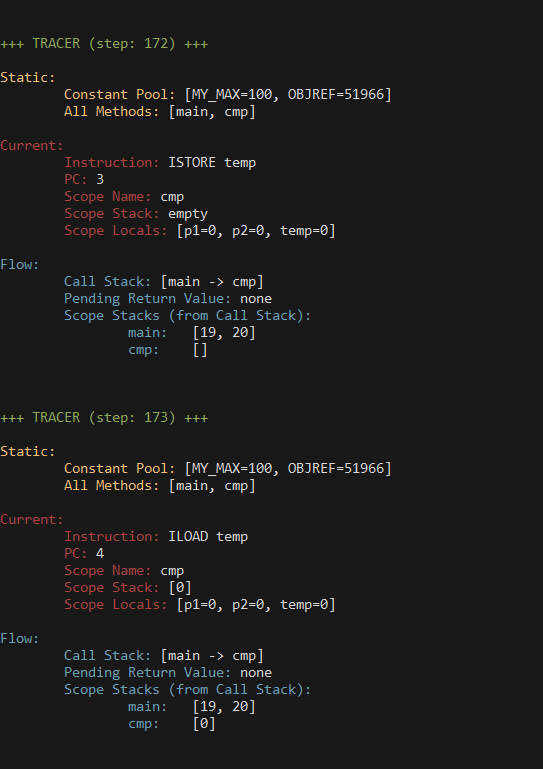
\includegraphics[width=0.8\textwidth]{images/terminal_trace_ijvm.png}
    \caption{IJVM tracer output example}
    \label{fig:terminal_trace_ijvm}
\end{figure}

\begin{figure}[H]
    \centering
    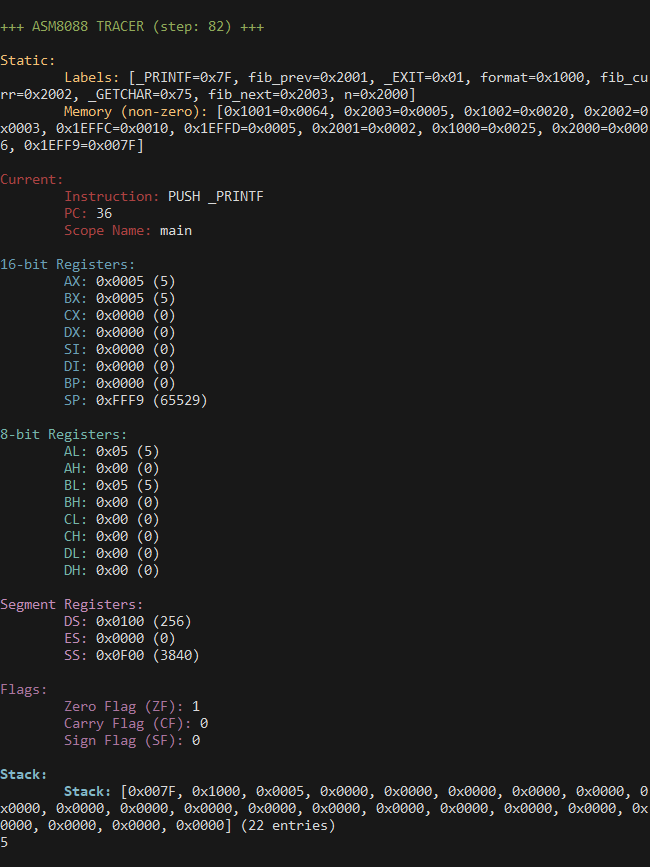
\includegraphics[width=0.8\textwidth]{images/terminal_trace_8088.png}
    \caption{8088 tracer output example}
    \label{fig:terminal_trace_8088}
\end{figure}

\section{Implementation Details}
The entire software has been implemented in Java 11, with a focus on modularity and extensibility. The following subsections cover key implementation details for the primary components.

\subsection{Lexers and Parsers}
In the following section, language names refer to their respective lexer/parser. For example, "IJVM" refers to [the lexer/parser of] IJVM, and "8088" refers to [the lexer/parser of] 8088.

The design features include:

\begin{itemize}
\item \textbf{Case Insensitivity}: All instructions accept both uppercase and lowercase representations, with the interpreter normalizing them to uppercase during processing.
\item \textbf{Flexible Number Formats}: Both lexers support multiple numeric representations. IJVM accepts decimal, hexadecimal (prefixed with \texttt{0x} or \texttt{0X}), and octal (prefixed with \texttt{o} or \texttt{O}) formats. 8088 supports decimal and hexadecimal formats with optional negative values.
\item \textbf{Identifier Rules}: Identifiers for variables, constants, methods, labels, and memory references start with a letter or underscore, followed by alphanumeric characters, underscores, or hyphens (IJVM only).
\item \textbf{Whitespace and Comment Handling}: Both IJVM and 8088 ignore whitespace and support comments using \texttt{//} and \texttt{;} styles. Newlines are explicitly tokenized to assist with block delimitation and error reporting.
\item \textbf{Language-Specific Keywords}: IJVM recognizes block delimiters like \texttt{.constant}, \texttt{.end-constant}, \texttt{.main}, \texttt{.end-main}, \texttt{.method}, \texttt{.end-method}, \texttt{.var}, and \texttt{.end-var} for program organization. 8088 includes section directives (\texttt{.SECT}, \texttt{.DATA}, \texttt{.TEXT}, \texttt{.BSS}) and data directives (\texttt{.BYTE}, \texttt{.ASCII}, \texttt{.SPACE}).
\item \textbf{Register Recognition}: 8088 explicitly recognizes 16-bit registers (AX, BX, CX, DX, SI, DI, BP, SP), 8-bit registers (AL, AH, BL, BH, CL, CH, DL, DH), and segment registers (CS, DS, ES, SS) as distinct tokens.
\item \textbf{Instruction Set Coverage}: IJVM tokens cover stack operations, arithmetic instructions, control flow, and method invocation. 8088 includes instruction coverage for data transfer, arithmetic operations, logical operations, and extensive conditional jump instructions.
\item \textbf{Memory Addressing Support}: 8088 includes brackets, parentheses, and arithmetic operators to support complex memory addressing modes with base registers, index registers, and displacement calculations.
\end{itemize}

The parsers use these tokens to create abstract syntax trees with hierarchical structures appropriate to each language. IJVM programs are organized into well-defined blocks (constant, main, method, var) with clear separation between execution code and declarations. 8088 handles section-based organization with separate processing for executable code (the \texttt{TEXT} section), initialized data (the \texttt{DATA} section), and uninitialized memory reservations (the \texttt{BSS} section).

\subsection{Semantic Analysis}
The semantic analyzer for both the language adopt a multi-pass analysis of the content; they extend ANTLR's base visitor pattern to traverse the AST and enforce semantic validation. 

In the following subsections, language names refer to their respective analyzers. For example, "IJVM" refers to [the semantic analyzer of] IJVM, and "8088" refers to [the semantic analyzer of] 8088.

\subsubsection{Multi-Pass Analysis Architecture}
IJVM processes declarations first, then scans labels for forward reference resolution, and then performs the semantic validation. 8088 follows a similar pattern but prioritizes the section-based organization and the register-instruction compatibility.

IJVM's first pass processes constant blocks and method declarations, registering all methods with their parameter lists. During the second pass, it collects all label declarations within each method scope, storing them in the \texttt{methodLabels} map for forward reference validation. After these two initialization passes, the third one performs the main analysis, checking variable initialization, method parameter compatibility, and control flow correctness.

8088's declaration pass focuses on constants and symbol registration, while the label scan pass collects all labels for jump instruction validation. The third pass works on register-instruction compatibility, section-directive alignment, and expression symbol resolution. Then finally, one last check is ran to search for undefined symbols.

\subsubsection{Instruction-Specific Validation}
IJVM implements stack simulation to validate stack operations. It maintains a \texttt{stackSize} counter that tracks the virtual stack depth, detecting stack underflow conditions for operations like \texttt{POP}, \texttt{SWAP}, and arithmetic instructions. Conditional jumps are validated for required stack operands, for example, \texttt{IFEQ} and \texttt{IFLT} requires one value, \texttt{IF\_ICMPEQ} requires two values. Method invocation validation ensures sufficient stack values for parameters plus an object reference. Variable access instructions (\texttt{ILOAD}, \texttt{ISTORE}) check variable declaration and initialization status. The analyzer also enforces control flow requirements, ensuring methods end with \texttt{IRETURN} instructions and detecting unreachable code after return statements.

8088 implements register-instruction compatibility checking. It maintains sets of byte instructions (\texttt{MOVB}, \texttt{ADDB}, \texttt{CMPB}) and byte registers (\texttt{AL}, \texttt{AH}, \texttt{BL}, \texttt{BH}) to enforce size matching. Byte instructions must use byte registers, while word instructions require word registers. The system also validates jump instruction placement within appropriate sections and directive-section compatibility.

\subsubsection{Misc Checks}
IJVM ensures \texttt{.var} blocks appear before any instructions within methods or main blocks, preventing variable declarations after executable code. It tracks instruction execution state using an \texttt{instructionsStarted} flag to enforce this ordering.

8088 validates section-directive relationships, ensuring \texttt{.BYTE} and \texttt{.ASCII} directives appear in \texttt{.DATA} sections, while \texttt{.SPACE} directives are permitted in both \texttt{.DATA} and \texttt{.BSS} sections. Jump instructions generate warnings when used outside \texttt{.TEXT} sections.

\subsubsection{Error Classification and Reporting} 
The semantic analysis framework distinguishes between errors and warnings via the \texttt{SemanticError} and \texttt{SemanticWarning} classes. Errors represent fatal semantic violations that prevent execution, such as undefined (but used) variables, type mismatches, or missing method returns. Warnings indicate potential but not-always-fatal issues such as potentially unreachable code blocks.

Error reporting includes precise source location information with line numbers and token positions, enabling users to quickly locate and resolve issues. The system provides descriptive error messages that attempt to explain both the problem and its context, such as \texttt{"Variable 'count' may not have been initialized before use"} or \texttt{"Byte instruction requires byte register, found 'AX'"}.

\subsection{Supported Instructions}
\begin{table}[H]
\caption{Supported IJVM Instructions}
\label{tab:instructions-ijvm}
\centering
\resizebox{\textwidth}{!}{
\begin{tabular}{|l|l|l|}
\hline
\textbf{Instruction} & \textbf{Description} & \textbf{Operands} \\
\hline
HALT            		& Terminates program execution                      				& None \\
NOP             		& No operation                         								& None \\
IADD            		& Adds the top two integers on the stack            			& None \\
ISUB            		& Subtracts the top integer from the second         			& None \\
IAND            		& Performs bitwise AND on the top two integers      		& None \\
IOR             		& Performs bitwise OR on the top two integers       			& None \\
POP             		& Removes the top element from the stack            			& None \\
SWAP            	& Swaps the top two elements on the stack           			& None \\
DUP             		& Duplicates the top element on the stack           			& None \\
ERR             		& Simulates an error                   								& None \\
IN              		& Simulates input reading                           					& None \\
OUT             		& Outputs the top stack value                       				& None \\
IRETURN         	& Returns from a method with the top stack value 			& None \\
BIPUSH          	& Pushes a byte value onto the stack                				& Integer \\
IINC            		& Increments a local variable by a value            				& Variable ID, Integer \\
ILOAD           		& Loads a variable value onto the stack             				& Variable ID \\
ISTORE          		& Stores the top stack value into a variable        				& Variable ID \\
INVOKEVIRTUAL & Invokes a method                                  					& Method ID \\
LDC\_W          	& Loads a constant value onto the stack             			& Constant ID \\
IFLT            		& Jumps if the top stack value is less than 0       			& Label ID \\
IFEQ            		& Jumps if the top stack value equals 0             				& Label ID \\
IF\_ICMPEQ      	& Jumps if the top two stack values are equal       			& Label ID \\
GOTO            		& Unconditionally jumps to a label                 				& Label ID \\
\hline
\end{tabular}
}
\end{table}

\newpage
\begin{table}[H]
\caption{Supported 8088 Instructions}
\label{tab:instructions-8088}
\centering
\footnotesize
\renewcommand{\arraystretch}{0.9}
\resizebox{\textwidth}{!}{
\begin{tabular}{|l|l|l|}
\hline
\textbf{Instruction} & \textbf{Description} & \textbf{Operands} \\
\hline
MOV & Moves data from source to destination & dest, src \\
MOVB & Moves byte data from source to destination & dest, src \\
PUSH & Pushes operand onto the stack & src \\
POP & Pops top of stack into operand & dest \\
ADD & Adds source to destination & dest, src \\
ADDB & Adds byte source to destination & dest, src \\
ADC & Adds source and carry flag to destination & dest, src \\
SUB & Subtracts source from destination & dest, src \\
SUBB & Subtracts byte source from destination & dest, src \\
SBB & Subtracts source and borrow from destination & dest, src \\
MUL & Multiplies AL by operand, result in AX & src \\
MULB & Multiplies AL by byte operand, result in AL/AH & src \\
DIV & Divides AX by operand, quotient in AL, remainder in AH & src \\
DIVB & Divides AL by byte operand, quotient in AL, remainder in AH & src \\
INC & Increments operand by 1 & dest \\
DEC & Decrements operand by 1 & dest \\
CMP & Compares destination with source & dest, src \\
CMPB & Compares byte destination with source & dest, src \\
AND & Performs bitwise AND & dest, src \\
OR & Performs bitwise OR & dest, src \\
XOR & Performs bitwise XOR & dest, src \\
XORB & Performs bitwise XOR on bytes & dest, src \\
NOT & Performs bitwise NOT & dest \\
JMP & Unconditional jump & label \\
JE/JZ & Jump if equal/zero & label \\
JNE/JNZ & Jump if not equal/not zero & label \\
JL/JNGE & Jump if less/not greater or equal & label \\
JLE/JNG & Jump if less or equal/not greater & label \\
JG/JNLE & Jump if greater/not less or equal & label \\
JGE/JNL & Jump if greater or equal/not less & label \\
JB/JNAE & Jump if below/not above or equal (unsigned) & label \\
JBE/JNA & Jump if below or equal/not above (unsigned) & label \\
JA/JNBE & Jump if above/not below or equal (unsigned) & label \\
JAE/JNB & Jump if above or equal/not below (unsigned) & label \\
JS/JNS & Jump if sign flag set/clear & label \\
JO/JNO & Jump if overflow flag set/clear & label \\
JP/JPE & Jump if parity flag set/parity even & label \\
JNP/JPO & Jump if no parity flag/parity odd & label \\
JC/JNC & Jump if carry flag set/clear & label \\
JCXZ & Jump if CX register is zero & label \\
LOOP & Loop while CX is not zero & label \\
CALL & Call subroutine & label \\
RET & Return from subroutine & None \\
SYS & System call & None \\
HLT & Halt execution & None \\
NOP & No operation & None \\
\hline
\end{tabular}
}
\end{table}

\newpage

\section{Usage}
The software can be executed as a CLI tool:

\begin{verbatim}
Usage: java -jar antlr-impl.jar [options]
Options:
  -parse, -interpret       Specify the mode
  -ijvm, -asm8088          Specify the language
  -file <path>             Path to the source file
  -d, -debug               Enable debug mode
  -trace                   Enable tracer
\end{verbatim}

\begin{itemize}
    \item \texttt{-parse}: Parse the specified file and report syntax and semantic errors.
    \item \texttt{-interpret}: Execute the specified file, provided no errors are found during parsing or semantic analysis.
    \item \texttt{-ijvm}: Specify the IJVM language.
    \item \texttt{-asm8088}: Specify the 8088 language.
    \item \texttt{-file <path>}: Path to the IJVM/8088 source file to interpret.
    \item \texttt{-d}, \texttt{-debug}: Enable debug mode for verbose output.
    \item \texttt{-trace}: Enable the tracer to view detailed step-by-step execution states, including memory dumps and stack contents.
\end{itemize}

\section{Testing}
Unit tests have been written to ensure that the parser, semantic analyzer, and interpreter are functioning as intended although some edge cases are omitted. These tests are found in the following classes:

\begin{itemize} 
	\item \texttt{IJVMProgramTest.java}: Evaluates the interpreter's computation of IJVM instructions, including arithmetic operations, stack management, control flow, and method calls. Test cases address scenarios such as stack underflow, variable initialization, and looping constructs. Additionally, executes a suite of tests from the \texttt{src/main/resources/examples} folder, which contains: tests from old course exams and the original Tanenbaum test case~\cite{ijvmtest}.
	\item \texttt{IJVMSemanticAnalyzerTest.java}: Ensures that the semantic analyzer finds errors such as uninitialized variables, undeclared method calls, invalid references, duplicate variable declarations, missing IRETURN statements, and stack underflow conditions. Also validates proper variable scoping and method parameter handling.
	\item \texttt{IJVMParserErrorTest.java}: Ensures the parser finds syntax issues, such as invalid instructions, missing block terminations, malformed method declarations, unclosed parentheses, invalid parameter separators, and missing colons in label declarations.
	\item \texttt{ASM8088ProgramTest.java}: Evaluates the interpreter's execution of 8088 assembly instructions, including movement operations, arithmetic instructions, comparison and flag operations, jump instructions, stack operations, logical operations, and memory addressing modes. Additionally, executes a suite of tests from the \texttt{src/main/resources/examples} folder containing AI-generated programs.
	\item \texttt{ASM8088SemanticAnalyzerTest.java}: Ensures that the semantic analyzer detects errors such as undefined symbols, register-instruction compatibility issues, section-directive mismatches, and improper code organization.
	\item \texttt{ASM8088ParserErrorTest.java}: Ensures the parser identifies syntax errors including invalid mnemonics, incorrect section directives, missing colons in label declarations, malformed memory addressing syntax, invalid constant formats, and improper directive syntax.
\end{itemize}

These tests increase confidence in the software correctness, but the implementation remains primarily an educational and experimental tool!

\newpage

\section{Summary}
This paper presents \texttt{antlr-impl}, an educational interpreter for subsets of the IJVM (Integer Java Virtual Machine) and Intel 8088 instruction sets, developed for the Computer Systems Architecture course at the University of Cagliari, built with Java 11 and ANTLR 4.

The tool implements a four-stage pipeline (Lexer, Parser, Semantic Analyzer, Interpreter) that work with both stack-based (IJVM) and register-based (8088) models.

Key features include a sophisticated three-pass semantic analyzer that performs stack simulation for IJVM and register-instruction compatibility checking for 8088, error reporting with precise source locations, and a real-time tracing system that visualizes program execution states.

\section*{Acknowledgments}
The authors acknowledge the use of Claude (Anthropic) as an AI assistant for writing assistance and implementation support during the development of this work. All final work was independently verified by the authors.

\bibliographystyle{unsrt}
\bibliography{references}

\end{document}
